\documentclass{ximera}

\graphicspath{{./}{thePythagoreanTheorem/}{deMoivreSavesTheDay/}{complexNumbersFromDifferentAngles/}}

\usepackage{tikz}
\usepackage{tkz-euclide}
\usetkzobj{all}
\tikzstyle geometryDiagrams=[ultra thick,color=blue!50!black]
\newcommand{\tri}{\triangle}
\renewcommand{\l}{\ell}
\renewcommand{\P}{\mathcal{P}}
\newcommand{\R}{\mathbb{R}}
\newcommand{\Q}{\mathbb{Q}}

\newcommand{\Z}{\mathbb Z}

\renewcommand{\vec}{\mathbf}
\renewcommand{\d}{\,d}



%% Egyptian symbols

\usepackage{multido}
\newcommand{\egmil}[1]{\multido{\i=1+1}{#1}{
\includegraphics[scale=.1]{egyptian/egypt_person.pdf}\hspace{0.5mm}}}
\newcommand{\eghuntho}[1]{\multido{\i=1+1}{#1}{
\includegraphics[scale=.1]{egyptian/egypt_fish.pdf}\hspace{0.5mm}}}
\newcommand{\egtentho}[1]{\multido{\i=1+1}{#1}{
\includegraphics[scale=.1]{egyptian/egypt_finger.pdf}\hspace{0.5mm}}}
\newcommand{\egtho}[1]{\multido{\i=1+1}{#1}{
\includegraphics[scale=.1]{egyptian/egypt_lotus.pdf}\hspace{0.5mm}}}
\newcommand{\eghun}[1]{\multido{\i=1+1}{#1}{
\includegraphics[scale=.1]{egyptian/egypt_scroll.pdf}\hspace{0.5mm}}}
\newcommand{\egten}[1]{\multido{\i=1+1}{#1}{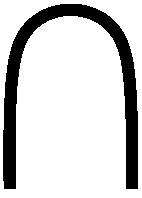
\includegraphics[scale=.1]{egyptian/egypt_heel.pdf}\hspace{0.5mm}}}
\newcommand{\egone}[1]{\multido{\i=1+1}{#1}{
\includegraphics[scale=.1]{egyptian/egypt_stroke.pdf}\hspace{0.5mm}}}
\newcommand{\egyptify}[7]{
 \multido{\i=1+1}{#1}{
\includegraphics[scale=.1]{egyptian/egypt_person.pdf}\hspace{0.5mm}}
 \multido{\i=1+1}{#2}{
\includegraphics[scale=.1]{egyptian/egypt_fish.pdf}\hspace{0.5mm}}
 \multido{\i=1+1}{#3}{
\includegraphics[scale=.1]{egyptian/egypt_finger.pdf}\hspace{0.5mm}}
 \multido{\i=1+1}{#4}{
\includegraphics[scale=.1]{egyptian/egypt_lotus.pdf}\hspace{0.5mm}}
 \multido{\i=1+1}{#5}{
\includegraphics[scale=.1]{egyptian/egypt_scroll.pdf}\hspace{0.5mm}}
 \multido{\i=1+1}{#6}{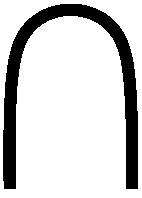
\includegraphics[scale=.1]{egyptian/egypt_heel.pdf}\hspace{0.5mm}}
 \multido{\i=1+1}{#7}{
\includegraphics[scale=.1]{egyptian/egypt_stroke.pdf}\hspace{0.5mm}}
 \hspace{.5mm}
}




\title{Euclid's Elements}

\begin{document}
\begin{abstract}
Here we see the beginning and some selections from
Euclid's \textit{Elements}.
\end{abstract}
\maketitle


Here is an excerpt from Euclid's \textit{Elements}. We have adapted
this from the edition by Richard
Fitzpatrick\link{http://farside.ph.utexas.edu/books/Euclid/Euclid.html}.




{\setlength{\parindent}{0pt}
\subsection*{Definitions}

1.~A point is that of which there is no part.

2.~And a line is a length without breadth.

3.~And the extremities of a line are points.

4.~A straight-line is (any) one which lies  evenly with points on itself.

5.~And a surface is that which has length and breadth only.

6.~And the extremities of a surface are lines.

7.~A plane surface is (any) one which lies evenly with the straight-lines on itself.

8.~And a plane angle is the inclination of the lines to one another, when two lines in a plane 
meet one another, and are not lying in a straight-line.

9.~And when the lines containing the angle are straight then the angle is called rectilinear.

10.~And when a straight-line stood upon (another) straight-line makes adjacent angles (which are) equal to one another, each of the equal angles is a
right-angle, and the former straight-line  is called a perpendicular to that upon which it stands.

11.~An obtuse angle is one greater than a right-angle.

12.~And an acute angle (is) one less than a right-angle.

13.~A boundary is that which is the extremity of something.

14.~A figure is that which is contained by some boundary or boundaries.

15.~A circle is a plane figure  contained by a single line [which is called a circumference], (such that) all of the straight-lines  radiating towards
 [the circumference] from one
point amongst those lying inside the figure  are equal to one another.

16.~And the point is called the center of the circle.

17.~And a diameter of the circle is any straight-line, being drawn through the
center, and terminated in each direction by the circumference of the circle. (And) any such (straight-line) also cuts the circle in half.$^\dag$

18.~And a semi-circle is the figure contained by the diameter  and
the circumference  cuts off by it. And the center of the semi-circle is the same (point)
as (the center of) the circle.

19.~Rectilinear figures are those (figures) contained by straight-lines: trilateral
figures being those contained by three straight-lines,  quadrilateral   by four,
and multilateral by more than four.

20.~And of the trilateral figures: an equilateral triangle is that having
three equal sides, an isosceles (triangle) that having only two equal sides,
and a scalene (triangle) that having three unequal sides.

21.~And further of the trilateral figures: a right-angled triangle is that having
a right-angle, an obtuse-angled  (triangle) that having an obtuse
angle, and an acute-angled (triangle) that having three acute angles.

22.~And of the quadrilateral figures: a square is that which is right-angled
and equilateral, a rectangle that which is right-angled but not equilateral,
a rhombus that which is equilateral but not right-angled, and a rhomboid that
having opposite sides and angles equal to one another which is neither
right-angled nor equilateral. And let quadrilateral figures besides these be called
trapezia.

23.~Parallel lines are straight-lines which, being in the same plane, and
being produced to infinity in each direction, meet with one another in
neither (of these directions).

\subsection*{Postulates}

1.~Let it have been postulated to draw a straight-line from any point to any point.

2.~And to produce a finite straight-line continuously in a straight-line.

3.~And to draw a circle with any center and radius.

4.~And that all right-angles are equal to one another.

5.~And that if a straight-line falling across two (other) straight-lines makes 
internal angles on the same side (of itself whose sum is) less than two right-angles, then the two (other) straight-lines, being produced to infinity, meet on that side (of the original straight-line) that the (sum of the internal angles) is less
than two right-angles (and do not meet on the other side).



\subsection*{Common Notions}

1.~Things equal to the same thing are also equal to one another.

2.~And  if equal things are added to equal things then the wholes are equal.

3.~And if equal things are subtracted from equal things then the remainders are
equal.

4.~And things coinciding with one another are equal to one another.

5.~And the whole [is] greater than the part.

}


\begin{proposition}[I.15]
If two straight-lines cut one another then they make the vertically
opposite angles equal to one another.
\end{proposition}

\begin{question}
Can you prove Proposition I.15?
\end{question}

\begin{proposition}[I.16]
For any triangle, when one of the sides is produced, the external
angle is greater than each of the internal and opposite angles.
\begin{image}
\begin{tikzpicture}[geometryDiagrams]
\coordinate (A) at (0,2);
\coordinate (B) at (2,5);
\coordinate (C) at (6.5,2);
\coordinate (F) at (9,2);
\draw (A)--(B)--(C)--cycle;
\draw (C)--(F);
\tkzLabelPoints[above](B)
\tkzLabelPoints[below](A,C)
\tkzMarkAngle[size=0.5cm,thin](F,C,B)
\tkzLabelAngle[pos = 0.25](F,C,B){$\epsilon$}

\tkzMarkAngle[size=0.6cm,thin](A,B,C)
\tkzLabelAngle[pos = 0.35](A,B,C){$\beta$}

\tkzMarkAngle[size=0.6cm,thin](C,A,B)
\tkzLabelAngle[pos = 0.35](C,A,B){$\alpha$}

%\draw[step=.5cm] (0,0) grid (10,5);
\end{tikzpicture}
\end{image}
\end{proposition}

\begin{question}
Can you prove Proposition I.16?
\end{question}

\begin{proposition}[I.27]
If a straight-line falling across two straight-lines makes the
alternate angles equal to one another then the (two) straight-lines
will be parallel to one another.
\end{proposition}


\begin{question}
Can you prove Proposition I.27?
\end{question}


\begin{proposition}[I.29]
A straight-line falling across parallel straight-lines makes the
alternate angles equal to one another, the external (angle) equal to
the internal and opposite (angle), and the (sum of the) internal
(angles) on the same side equal to two right-angles.
\end{proposition}


\begin{question}
Can you prove Proposition I.29?
\end{question}


\begin{proposition}[I.32]
In any triangle, (if) one of the sides (is) produced (then) the
external angle is equal to the (sum of the) two internal and opposite
(angles), and the (sum of the) three internal angles of the triangle
is equal to two right-angles.
\end{proposition}


\begin{question}
Can you prove Proposition I.32?
\end{question}
\end{document}
